\documentclass{beamer}

% You can also use a 16:9 aspect ratio:
%\documentclass[aspectratio=169]{beamer}
\usetheme{TACC16}

% It's possible to move the footer to the right:
%\usetheme[rightfooter]{TACC16}

\begin{document}
\title[Lmod/XALT]{Lmod and XALT}
\author{Robert McLay} 
\date{November 14, 2018} 

% page 1
\frame{\titlepage} 

% page 2
\begin{frame}{Lmod: A Modern Replacement for Env. Modules}
  \begin{itemize}
    \item Reads TCL and Lua modulefiles
    \item Support Software Hierarchy, but not required!!
    \item Spider Cache: Fast loads, avail, spider
    \item Sites can have hidden modules.
    \item Optional Tracking of Module Usage.
    \item Many more features: https://lmod.readthedocs.io
  \end{itemize}
\end{frame}

% page 3
\begin{frame}[fragile]
    \frametitle{Lmod Doc usage}
    \center{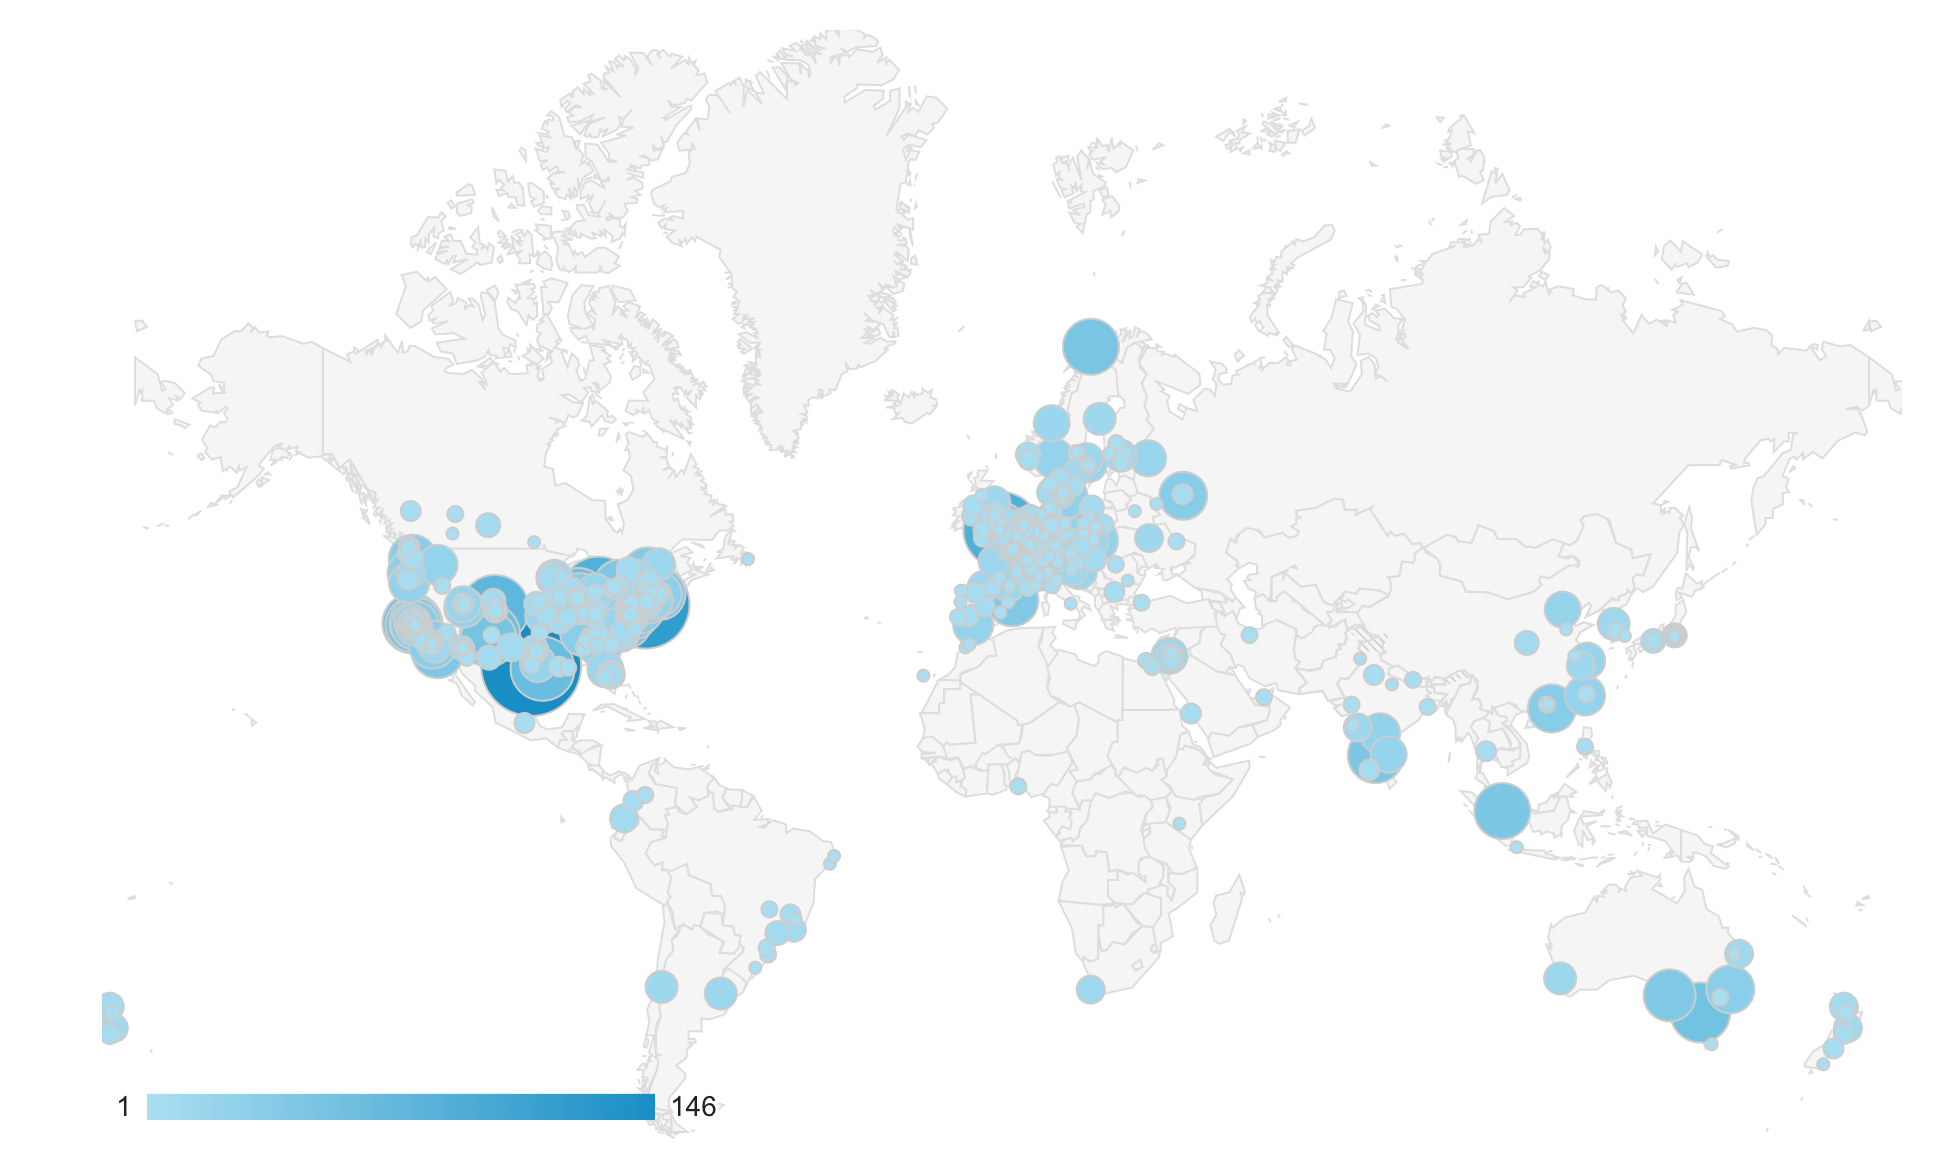
\includegraphics[width=.9\textwidth]{Lmod_docs_usage}}
\end{frame}

% page 4
\begin{frame}{XALT: Tracks what executables and libraries that are run}
  \begin{itemize}
    \item Tracks both MPI and Non-MPI (Scalar/serial) programs
    \item Tracks run time and library usage
    \item Extremely light weight
    \item Scalar programs are sampled to prevent being overwhelmed.
    \item Not a performance tool.
  \end{itemize}
\end{frame}

% page 5
\begin{frame}{XALT: Tracking Tool}
  \begin{itemize}
    \item Site Configurable
    \item Optionally Track Package use in R, MATLAB, and Python
    \item Used to know resource usage by Node-Hours, How Frequent,
      Most Users.
    \item Learn more at: xalt.readthedocs.io
  \end{itemize}
\end{frame}

%\input{./themes/license}

\end{document}
